\documentclass{beamer}

\usetheme{Juelich}

\usepackage{tikz}
\usetikzlibrary{shapes.geometric}
\usetikzlibrary{calc, matrix}
\usetikzlibrary{decorations.pathmorphing}
\pgfdeclarelayer{bg}   
\pgfsetlayers{bg,main}

\usepackage{fancyvrb}
\fvset{fontfamily=courier,fontsize=\scriptsize,commandchars=|^~}
\newcommand*{\fvtextcolor}[2]{\textcolor{#1}{#2}}

\title{LEAP School Project\\ Simple Many Body Code}
\author{T. Hater}
\institute{FZJ | JSC | PADC}
\date{\today}

\begin{document}
\begin{frame}[fragile]{The Problem}
    \begin{columns}
    \begin{column}{0.35\textwidth}
      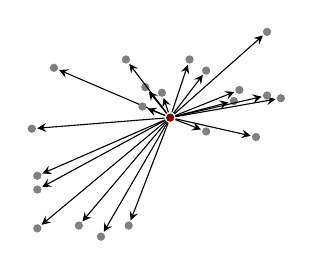
\begin{tikzpicture}[ >=stealth, ->, draw=black, fill=black]
        \foreach \i in {0, ..., 20} {
          \pgfmathrandominteger{\x}{-50}{50}
          \pgfmathrandominteger{\y}{-50}{50}
          \fill[gray] (\x pt, \y pt) circle (1.5pt);
          \draw[<-,shorten >=2pt, shorten <=2pt] (\x pt, \y pt) -- (0,0);
        }
        \fill[red!50!black] (0,0) circle (1.5pt);
      \end{tikzpicture}
    \end{column}
    \begin{column}{0.45\textwidth}
      \begin{itemize}
      \item $N$ Particles of mass $m$, initially
        in unit box $[0,1)^3$.
      \item Direct $\mathcal{O}(N^2)$ evaluation of gravitation 
        \begin{equation*}
          \mathbf{F}_i = \sum_{i\neq j} Gm^2\frac{\mathbf{r}_i - \mathbf{r}_j}{|\mathbf{r}_i - \mathbf{r}_j|^3}
        \end{equation*}
      \item Equation of motion 
        \begin{equation*}
          m\ddot{\mathbf{r}}_i = \mathbf{F}_i
        \end{equation*}
      \item Simple timestepping
      \end{itemize}
    \end{column}
  \end{columns}
\end{frame}

\begin{frame}{Project Outline and Goals}
  \begin{enumerate}
  \item Analysing the code
  \item Porting to NVIDIA GPUs using CUDA
  \item Understanding and optimising accelerator performance
    \begin{itemize}
    \item Shared memory, coalescing and memory organisation
    \item Profilers and hardware performance counters
    \end{itemize}
  \item Developing an optimised implementation on the CPU
    \begin{itemize}
    \item Caches, multithreading and vectorisation
    \item Hardware performance counters on the CPU
    \end{itemize}
  \item Comparing two platforms: CPU vs GPU
  \end{enumerate}
\end{frame}
\end{document}
